\documentclass[border={0.1cm 0.1cm 0.1cm 0.1cm}]{standalone}  %E,S,W,N

\usepackage{amssymb}
\usepackage{amsmath}
\usepackage{tikz}
\usetikzlibrary{decorations.pathreplacing}	%for brackets

\begin{document}
	
	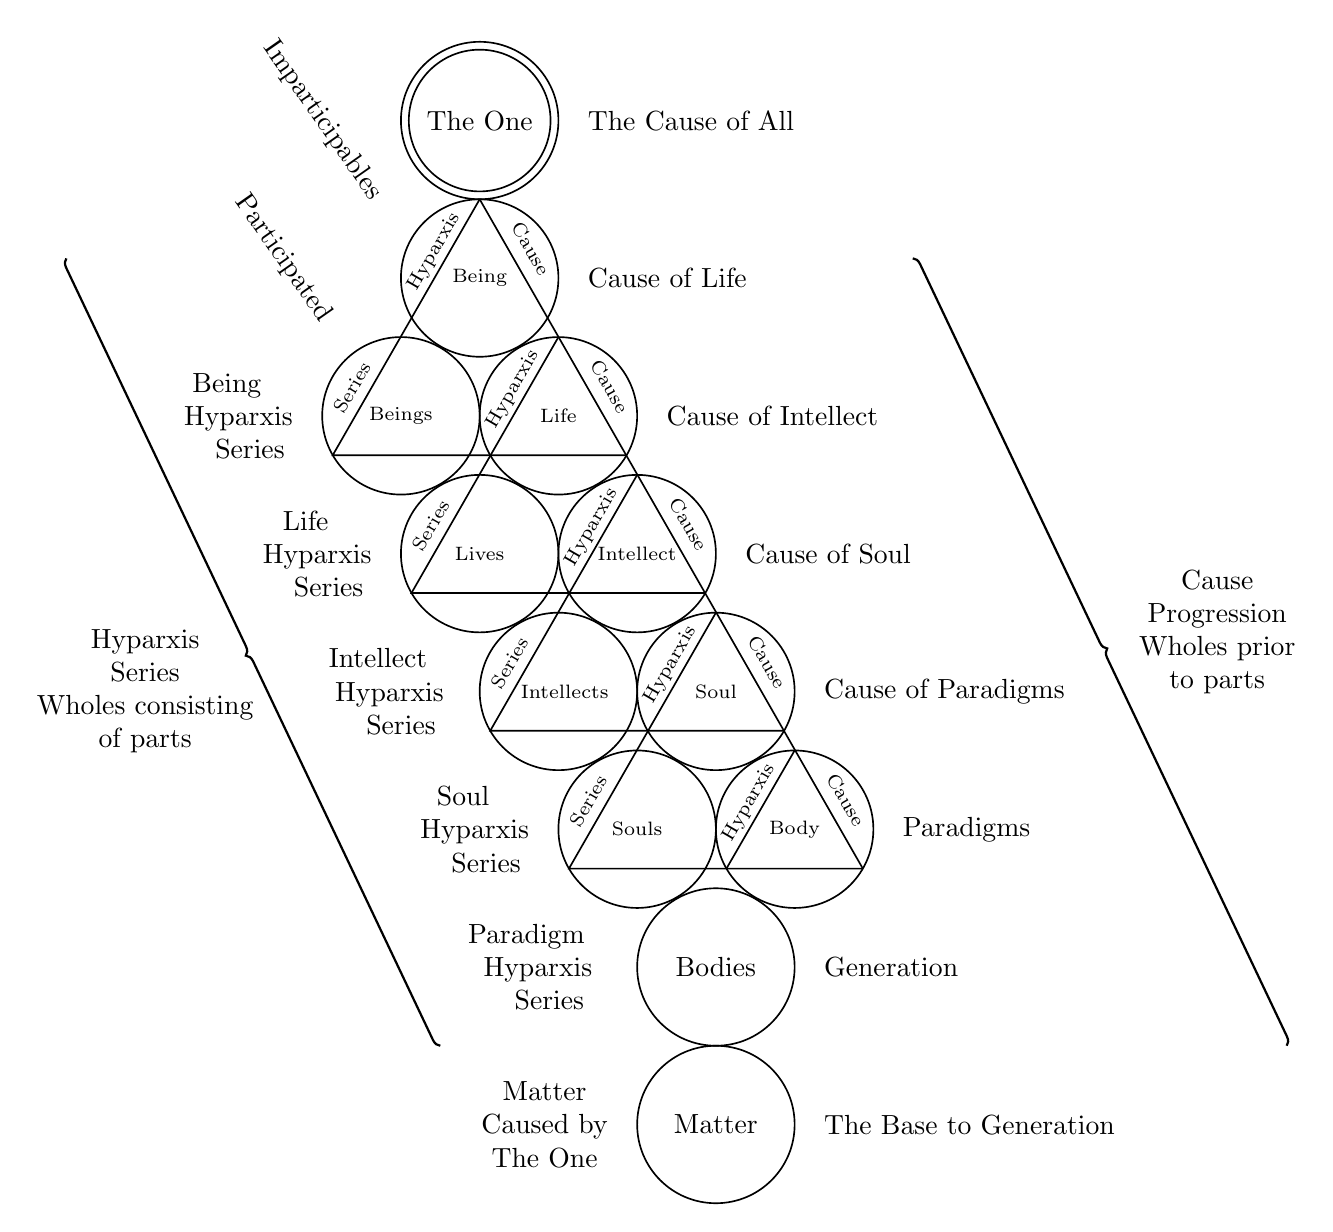
\begin{tikzpicture}	
	%CIRCLES
	\node at (-5,12.75) {\rotatebox{-55}{Imparticipables}};
	\node at (-5.5,11) {\rotatebox{-55}{Participated}};
	%
	\draw[semithick] (-3,12.75) circle (1cm) circle (0.9cm) node {The One};
		\node[align=left,right] at (-1.75,12.75) {The Cause of All};
	\draw[semithick] (-3,10.75) circle (1cm) node {\scriptsize Being};
		\node[align=left,right] at (-1.75,10.75) {Cause of Life};
	%
	\draw[semithick] (-4,9) circle (1cm) node {\scriptsize Beings};
		\node[align=center,left] at (-5.25,9) {Being$\;\;\;$\\Hyparxis\\$\;\;\;$Series};
	\draw[semithick] (-2,9) circle (1cm) node {\scriptsize Life};
		\node[align=left,right] at (-0.75,9) {Cause of Intellect};
	%
	\draw[semithick] (-3,7.25) circle (1cm) node {\scriptsize Lives};
		\node[align=center,left] at (-4.25,7.25) {Life$\;\;\;$\\Hyparxis\\$\;\;\;$Series};
	\draw[semithick] (-1,7.25) circle (1cm) node {\scriptsize Intellect};
		\node[align=left,right] at (0.25,7.25) {Cause of Soul};
	%
	\draw[semithick] (-2,5.5) circle (1cm) node {\scriptsize $\;\;$Intellects};
		\node[align=center,left] at (-3.25,5.5) {Intellect$\;\;\;$\\Hyparxis\\$\;\;\;$Series};
	\draw[semithick] (0,5.5) circle (1cm) node {\scriptsize Soul};
		\node[align=left,right] at (1.25,5.5) {Cause of Paradigms};
	%
	\draw[semithick] (-1,3.75) circle (1cm) node {\scriptsize Souls};
		\node[align=center,left] at (-2.25,3.75) {Soul$\;\;\;$\\Hyparxis\\$\;\;\;$Series};
	\draw[semithick] (1,3.75) circle (1cm) node {\scriptsize Body};
		\node[align=left,right] at (2.25,3.75) {Paradigms};
	%
	\draw[semithick] (0,2) circle (1cm) node {Bodies};
		\node[align=center,left] at (-1.25,2) {Paradigm$\;\;\;$\\Hyparxis\\$\;\;\;$Series};
		\node[align=left,right] at (1.25,2) {Generation};
	\draw[semithick] (0,0) circle (1cm) node {Matter};
		\node[align=left,right] at (1.25,0) {The Base to Generation};
		\node[align=center,left] at (-1.25,0) {Matter\\Caused by\\The One};
	
	%TRIANGLE PARTS
	\draw[semithick] ({-3+cos(90)},{10.75+sin(90)})--({1+cos(-30)},{3.75+sin(-30)});
	\draw[semithick] ({1+cos(210)},{3.75+sin(210)})--({1+cos(90)},{3.75+sin(90)});
	
	%INNER LABELS
	\foreach \i in {0,...,3}{
	\draw[semithick] ({-1*\i+1+cos(-30)},{1.75*\i+3.75+sin(-30)})-- ({-1*\i-1+cos(210)},{1.75*\i+3.75+sin(210)})--({-1*\i+cos(90)},{1.75*\i+5.5+sin(90)});
	\node at ({-1*\i+1+0.75*cos(30)},{1.75*\i+3.75+0.75*sin(30)}) {\rotatebox{-60}{\scriptsize Cause}};
	\node at ({-1*\i+1+0.67*cos(150)},{1.75*\i+3.75+0.67*sin(150)}) {\rotatebox{60}{\scriptsize Hyparxis}};
	\node at ({-1*\i-1+0.72*cos(150)},{1.75*\i+3.75+0.72*sin(150)}) {\rotatebox{60}{\scriptsize Series}};
	}
	%STRAGGLERS
	\node at ({-1*4+1+0.75*cos(30)},{1.75*4+3.75+0.75*sin(30)}) {\rotatebox{-60}{\scriptsize Cause}};
	\node at ({-1*4+1+0.67*cos(150)},{1.75*4+3.75+0.67*sin(150)}) {\rotatebox{60}{\scriptsize Hyparxis}};
	
	%BRACES
	\draw[decorate,decoration={brace,amplitude=3pt},thick] (-3.5,1)--(-8.25,11);
		\node[align=center,left] at (-5.75,5.5) {Hyparxis\\Series\\Wholes consisting\\of parts};
	\draw[decorate,decoration={brace,amplitude=3pt},thick] (2.5,11)--(7.25,1);
		\node[align=center,right] at (5.25,6.25) {Cause\\Progression\\Wholes prior\\to parts};
	
	%\draw[help lines] (-8,-2) grid (8,13);
	\end{tikzpicture}
	
\end{document}